\section{Introduction}\label{sec:intro}
The RabbitMQ FMU is an implementation of an external data broker based on
RabbitMQ. The RabbitMQ FMU subscribes to a RabbitMQ queue and publishes the
message content via its outputs. This way, the RabbitMQ FMU brings data from any source into an
FMI simulation context. Note, that this document assumes general knowledge of
the Functional Mock-up Interface.

The approach is depicted in~\cref{fig:interfacing_overview}, where
the content within the \textit{System Specific} frame will vary based on the system
providing the data. The Log-Translator entity translates the
system-specific log messages to RabbitMQ messages and publishes them to a
RabbitMQ queue, which RabbitMQ FMU is configured to subscribe to. This means
that RabbitMQ FMU has some system-specific configuration, however this is
contained to the static model description file. RabbitMQ FMU then publishes the
RabbitMQ messages via regular FMI outputs.

\begin{figure}[htb]
  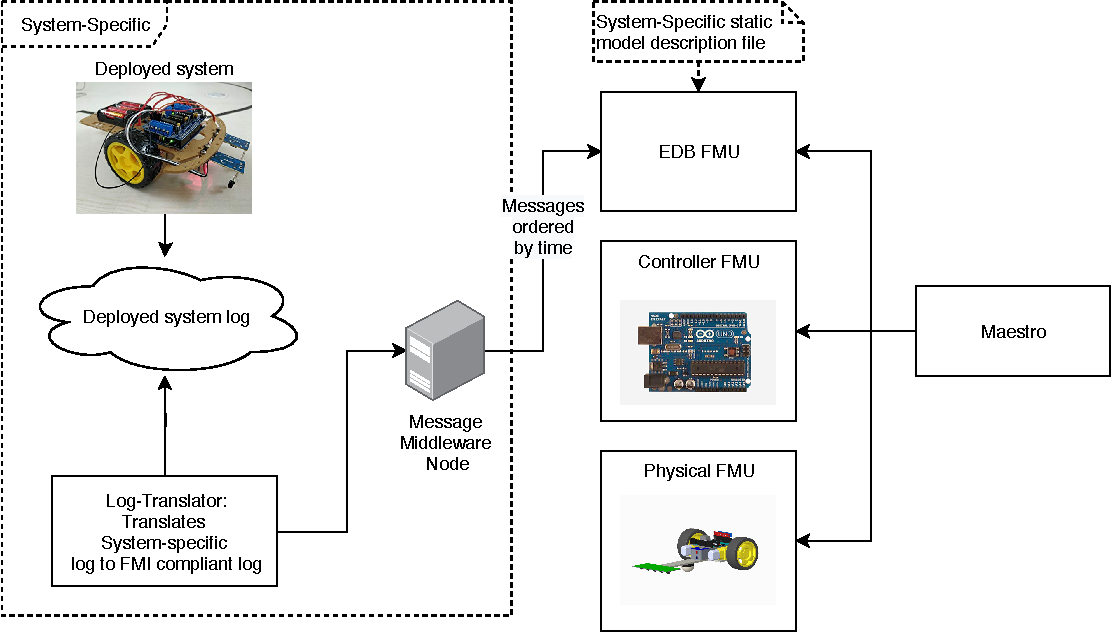
\includegraphics[width=\textwidth]{figures/overview.pdf}
  \caption{Interfacing Overview}
 \label{fig:interfacing_overview}
\end{figure}

This approach generalises the FMI enabling entity, the RabbitMQ FMU, such that
it can be used for different kinds of systems with different kinds of logging
facilities.
The motivation behind this approach is that tools of the INTO-CPS Association
should be generally applicable.

The following chapters describes the following in order:
\begin{description}
  \item[Time Handling] How system-time is mapped to time in an FMI-simulation
    context
  \item[Configuration] How to configure the FMU via the ModelDescription File
  \item[Example - Line Following Robot] This example demonstrates transmission
    of data from a deployed line following robot that is available in the
    co-simulation of its digital twin and how the values differ.
  \item[Conclusion] A brief conclusion on the contribution.
\end{description}


%%% Local Variables:
%%% mode: latex
%%% TeX-master: "../rabbitmq-fmu"
%%% End:
